\documentclass[10pt]{article}
\usepackage[margin=0.65in]{geometry}
\usepackage[T1]{fontenc}
\usepackage{lmodern}
\usepackage{microtype}
\usepackage{amsmath,amssymb}
\usepackage{booktabs,array,tabularx}
\usepackage{listings}
\usepackage{xcolor}
\usepackage[hidelinks]{hyperref}
\usepackage{enumitem}
\usepackage{titlesec}
\usepackage{tikz}
\usetikzlibrary{arrows.meta,positioning,calc}

\setlist{nosep,leftmargin=1.4em}
\titlespacing*{\section}{0pt}{1.1ex}{0.5ex}
\titlespacing*{\subsection}{0pt}{0.9ex}{0.3ex}
\setlength{\parskip}{0.3em}
\setlength{\parindent}{0pt}

\lstdefinestyle{code}{
  basicstyle=\ttfamily\footnotesize,
  columns=fullflexible,
  keepspaces=true,
  frame=single,
  rulecolor=\color{black!30},
  backgroundcolor=\color{black!3},
  xleftmargin=0.3em, xrightmargin=0.3em,
  aboveskip=0.4em, belowskip=0.2em,
  escapeinside={(*}{*)},
  breaklines=true
}
\lstset{style=code}
\newcommand{\code}[1]{\texttt{\small #1}}
% Draft marker: delete each one once the text is confirmed.
\newcommand{\todo}[1]{\textcolor{red!70!black}{\textbf{[TODO: #1]}}}

\title{\vspace{-1.2em}\textbf{P3 GC Design Note: Lisp-2 Sliding Mark-Compact (Rust Runtime)}\vspace{-0.4em}}
\author{Neha Reddy \quad Sarthak Dayal \quad Jay Shim \quad Rahik Sikder\\[0.2em] CS 378H, Fall 2026}
\date{}

\begin{document}
\maketitle
\vspace{-2.2em}

\section{Choice and Heap Layout}
We implemented the \emph{Lisp-2 sliding mark-compact} collector in the Rust skeleton. We chose it because it uses the whole heap rather than half, and because its difficulty sits in one place, the pointer-fixup discipline, which we could enumerate and test directly. The reference Cheney collector stays in \code{rust/reference/} behind the \code{reference-cheney} Cargo feature, so we can diff against it.
\begin{itemize}
  \item \textbf{Heap.} One contiguous region with a bump pointer \code{FREE}, 16~MiB by default and overridden by \code{LO\_HEAP\_SIZE} at \code{lo\_runtime\_init}. Objects sit end to end, so the allocated prefix $[\mathrm{base},\mathrm{FREE})$ can be walked linearly.
  \item \textbf{Allocation.} \code{lo\_alloc} bumps \code{FREE}. If the object does not fit, it forces one collection and retries once, aborting through \code{lo\_alloc\_oom} (exit 137) only if the live set still leaves no room.
  \item \textbf{Sizes and offsets.} All sizes come from \code{heap\_layout::object\_size} (\code{align(instance\_size)}, or \code{align(string\_data\_offset + length)} for a \code{String}), and every field offset comes from \code{offset\_of} or the descriptors. Nothing is hard-coded to the 16-byte native or 12-byte WASM header.
  \item \textbf{Mark bit.} Bit~0 of \code{gc\_bits}, clear between collections.
  \item \textbf{Side metadata.} Descriptors must stay intact throughout, since the heap walk reads them, so forwarding addresses are not stored in headers. \code{compaction::Scratch} instead holds a mark \code{worklist} and a table of \code{Relocation\{old\_offset, new\_offset, size\}}, both reserved \emph{at init} and never during a collection.
  \item \textbf{No allocation during collection.} A collection never allocates, and re-entry is rejected by an \code{IN\_COLLECTION} assertion.
  \item \textbf{Barrier.} \code{lo\_gc\_write\_barrier} stays the skeleton's bare store. With one generation there is no old-to-young pointer to miss, so no remembered set or card table is needed.
\end{itemize}

\section{Roots and Collection Passes}
The only roots are the shadow-stack slots. The collector walks the \code{ShadowFrame} chain from \code{current\_frame} and visits each frame's \code{num\_roots} slots, including the static \code{lo\_bindings} frame. Since P2's \code{gc\_roots} spills every live \code{Ref} around each call, no register or native-stack scan is needed. \code{managed(p)} is true iff $p$ is non-null and $\mathrm{base}\le p<\mathrm{FREE}$, and every visited pointer passes through it. \code{LO\_EMPTY\_STRING}, literals, and descriptors live in static data, so they are never marked, moved, or rewritten, with no special case. The ABI supplies object-start pointers only, so an exact-start lookup suffices.

\begin{center}\small
\begin{tabularx}{\linewidth}{@{}l X@{}}
\toprule
\textbf{Phase} & \textbf{What it does} \\
\midrule
\code{mark} & Marks from the roots with a worklist of heap offsets, so the traversal depth lives in the worklist rather than on the call stack and long link chains cannot overflow the stack. The mark bit is set before pushing, so cycles and aliases enter once. Fields come from the descriptor's \code{pointer\_offsets}, which need not be contiguous. \\
\code{compute\_forwarding} & Walks the heap with \code{object\_size}. Each marked object gets \code{new\_offset} equal to the live bytes before it. Entries are appended in address order, so the table is sorted by construction. \\
\code{fix\_references} & Rewrites every root slot and every pointer field of every live object, looking the target object up by binary search. All fixups run while every object is still at its old address. \\
\code{slide} & Copies objects down in ascending order with the overlap-safe \code{ptr::copy}, clearing mark bits. Since $\mathrm{new}\le\mathrm{old}$ for every object, no unmoved object is overwritten. \\
\bottomrule
\end{tabularx}
\end{center}
Afterward \code{FREE} is set to the end of the live prefix. With \code{LO\_GC\_POISON=1} the freed tail is filled with \code{0xEF}, so a stale pointer fails loudly.

\begin{center}
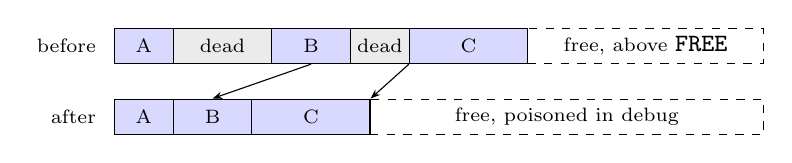
\begin{tikzpicture}[font=\scriptsize, x=0.5cm,
  live/.style={draw, fill=blue!15, minimum height=0.45cm, inner sep=0pt},
  dead/.style={draw, fill=black!8, minimum height=0.45cm, inner sep=0pt},
  free/.style={draw, dashed, minimum height=0.45cm, inner sep=0pt},
  mv/.style={-{Stealth[length=3.5pt]}, thin}]
\node[anchor=east] at (-0.2, 0) {before};
\node[live, minimum width=1.5*0.5cm, anchor=west] (a) at (0,0) {A};
\node[dead, minimum width=2.5*0.5cm, anchor=west] at (1.5,0) {dead};
\node[live, minimum width=2.0*0.5cm, anchor=west] (b) at (4.0,0) {B};
\node[dead, minimum width=1.5*0.5cm, anchor=west] at (6.0,0) {dead};
\node[live, minimum width=3.0*0.5cm, anchor=west] (c) at (7.5,0) {C};
\node[free, minimum width=6*0.5cm, anchor=west] at (10.5,0) {free, above \code{FREE}};
\node[anchor=east] at (-0.2, -0.9) {after};
\node[live, minimum width=1.5*0.5cm, anchor=west] at (0,-0.9) {A};
\node[live, minimum width=2.0*0.5cm, anchor=west] (b2) at (1.5,-0.9) {B};
\node[live, minimum width=3.0*0.5cm, anchor=west] (c2) at (3.5,-0.9) {C};
\node[free, minimum width=10*0.5cm, anchor=west] at (6.5,-0.9) {free, poisoned in debug};
\draw[mv] (b.south) -- (b2.north);
\draw[mv] (c.south west) -- (c2.north east);
\end{tikzpicture}
\end{center}

\textbf{Fixup argument.} After a collection no pointer may hold an old address, so we list every place a managed pointer can live and how each is handled.
\begin{enumerate}
  \item \textbf{Shadow-stack slots.} These are the roots, and \code{fix\_references} rewrites each to its object's new address.
  \item \textbf{Pointer fields of live objects.} Rewritten for \emph{every} live object, including ones that do not move, because an unmoved object can point at one that does.
  \item \textbf{Pointers outside the heap.} Descriptors, literals, and \code{LO\_EMPTY\_STRING} fail the \code{managed()} range check and are left alone. They never move, so their addresses are already correct.
  \item \textbf{Pointers held by the runtime itself.} There are none. String operations copy their inputs into a Rust \code{Vec} \emph{before} allocating, so no managed pointer is held across a possible collection. \code{lo\_cast\_check} and \code{lo\_instanceof} allocate nothing. The worklist and relocation table hold offsets, not pointers.
  \item \textbf{The bump pointer.} \code{FREE} is reset to the end of the live prefix.
\end{enumerate}
If these cover every location, nothing holds a stale address after \code{slide}. Dead objects are never visited, so their stale fields are never read.

\textbf{String and type operations.} The five \code{lo\_string\_*} operations are UTF-8 aware (codepoint-aware reversal, byte-wise comparison, exit 120 on a negative repeat count) and follow the root discipline above. \code{lo\_cast\_check} and \code{lo\_instanceof} walk the descriptor \code{parent} chain, with null short-circuits and exit 101 naming both classes.

\section{Testing on Both Targets}
\textbf{LO stress tests} (suite header-contract format) are in \code{tests/gc-stress/}. There are five, and each allocates about 3 million objects, keeps live data under a quarter of its heap, and was confirmed to fail on a copy of our runtime with the named bug planted.
\begin{center}\small
\begin{tabularx}{\linewidth}{@{}l X@{}}
\toprule
\textbf{Test} & \textbf{Invariant (planted bug it catches)} \\
\midrule
\code{gc\_01\_unmoved\_anchor\_fixup} & Fixup rewrites fields of unmoved live objects (fixup skips objects whose address is unchanged) \\
\code{gc\_02\_overlapping\_slide} & A slide shorter than the object is overlap-safe (copying high to low, or the tail block first) \\
\code{gc\_03\_survivors\_then\_die} & Survivors are reclaimed once dead (mark bits left set) \\
\code{gc\_04\_deep\_list\_marking} & Marking uses a worklist (recursive marking overflows the stack on a very long link chain) \\
\code{gc\_05\_every\_pointer\_field} & Scan visits exactly the descriptor's offsets (first field only, last field skipped, contiguity assumed) \\
\bottomrule
\end{tabularx}
\end{center}
\code{run.sh} runs each program on WASM and native at the default heap, and on native at its declared heap. All five pass on both targets, and natively at their declared heaps. A WASM module has no environment, so \code{LO\_HEAP\_SIZE} cannot reach it and WASM always runs at 16~MiB. There, collections come from allocating past that heap.

\textbf{Forced collections.} LO source has no way to call \code{lo\_gc\_collect}, which the ABI reserves for tests, so these programs force collections by exhausting the heap instead. Each allocates about 3 million short-lived objects against its declared heap, so collections recur throughout the run while the program's live data is in a known shape. Direct \code{lo\_gc\_collect} calls are exercised by Rust tests, run natively and compiled to WASM, which \code{tests/gc-stress/README.md} maps to each stress-test category.

\section{Challenges and Limitations}
\textbf{Tradeoffs.}
\begin{itemize}
  \item \textbf{Lisp-2 over Cheney.} We use the whole heap instead of half, but make three passes per collection instead of one copy.
  \item \textbf{Side tables over header forwarding.} Descriptors stay intact for the heap walk, but fixup needs a binary search per pointer rather than a direct read.
  \item \textbf{Scratch reserved at init.} A collection never allocates, but the tables reserve about twice the heap in address space.
  \item \textbf{Non-generational.} The barrier stays a bare store and nothing can be missed, but every collection scans all live data.
\end{itemize}
\textbf{Limitations.}
\begin{itemize}
  \item There is no heap-checker walk and no per-collection GC log, only poisoning.
  \item WASM always runs at the default 16~MiB heap, so small heaps are tested natively only.
  \item Out-of-memory inside \code{lo\_string\_repeat} still exits 120 on WASM, since \code{wasmrun} matches that name first.
\end{itemize}
\textbf{Bug found.} Heap exhaustion inside a string operation (\code{lo\_string\_concat}, \code{lo\_string\_new}, \code{lo\_string\_reverse}) exited 134 on WASM instead of the required 137 (native was correct). \code{wasmrun} picks a trap's exit code from its backtrace and reports 137 only if a \code{lo\_alloc*} frame is on it, but our string operations aborted from their own out-of-memory paths. Every out-of-memory abort now goes through one \code{\#[cold] \#[inline(never)] lo\_alloc\_oom}, which stays a real frame. \todo{Confirm this bug and add how it was found.}

\end{document}
